The next experiment we ran was to measure the amount of time it takes to run a procedure with 0-7 integer parameters. In addition, we measured the overhead for returning from a function call. We predict that a procedure call with no parameters should take two memory writes for the return address and the stack pointer, for an estimate of 52 cycles. Each parameter should add about 2 cycles for passing the argument through a register. We implement each experiment as follows: 
\begin{verbatim}
void function(int v1, int v2, ... int vn){
  GET_HIGH(end);
}

unsigned long measure(){
  int v1 = 1;
  int v2 = 2;
  ...
  int vn = n;
  GET_HIGH(start);
  function(v1,v2, ... vn);
  return end - start;
}
\end{verbatim}

\noindent Note that, for standardization purposes, arguments are loaded into variables and passed to the function through these variables. This way, we know that the data is local, in cache and in the TLB, and computing the values to be passed to the function takes the same amount of time. This method is used in later experiments, where procedure call overhead affects the measurement, and must be subtracted.
\newline
\newline
As for procedure return overhead, we predict that it should take a memory read to access the return address, as well as about 2 cycles to pass the return value to a register, for a total of 28 cycles. We implement the return overhead experiment as follows:
\begin{verbatim}
void function() {
  GET_HIGH(start);
}

unsigned long measure() {
  function();
  GET_HIGH(end);
  return end - start;
}
\end{verbatim}

\newpage

\noindent The overhead for a function call is plotted in the table below:
\newline
\newline
\begin{tabular}{c|c|c}

	\textbf{Parameters} & \textbf{Overhead (cycles)} & \textbf{St. Dev.} \\\hline
	0 & 16 & 0\\\hline
	1 & 19 & 0\\\hline
	2 & 24.004 & 0.33\\\hline
	3 & 23 & 0\\\hline
	4 & 28.002 & 0.11\\\hline
	5 & 32 & 0\\\hline
	6 & 33 & 0\\\hline
	7 & 37 & 0\\\hline

\end{tabular}
\newline
\newline

\begin{comment}
\begin{figure}[h]
\centering
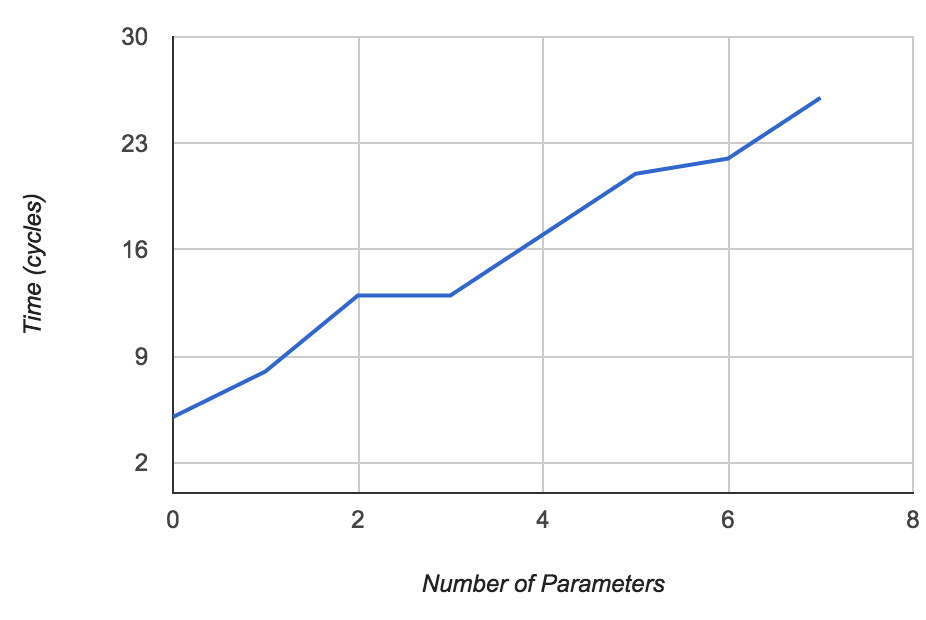
\includegraphics[scale=.5]{experiments/exp_1_2_fig.png}
\caption{Mean execution time vs number of parameters.  Overhead time included for comparison.  The standard deviation for all experiments was under 1 ns}
\end{figure}
\end{comment}

\noindent We see that the baseline overhead for a procedure call is actually 19 cycles. Again, our overestimates in memory access time caused us to significantly overestimate procedure call time. Again, dividing the memory estimates by 2, we get 13 cycles for a memory write, yielding an improved estimate of 28 cycles for a procedure call. However, this is still a significant overestimate, so we will need to review our understanding of this architecture's function call ABI. As for the overhead of each additional parameter, we were somewhat more accurate; on average, the additional overhead was 3 cycles per additional parameter. However, we observe anomalous nonlinear increase, and an actual decrease between 2 and 3 parameters. We speculate that this is due to out-of-order execution, which we will have to figure out how to avoid in the future.
\newline
\newline
The overhead for returning from a function call was consistently 16 cycles for each trial in the experiment. In the future, we should compare this with the overhead for actually returning a value from the function.